\documentclass[uplatex,dvipdfmx,10pt]{jsarticle}

\usepackage{amsmath,amssymb,mathtools}
\usepackage[top=16mm,bottom=16mm,left=18mm,right=18mm,headsep=5mm]{geometry}
\usepackage[dvipdfmx,hidelinks]{hyperref}
\usepackage{pxjahyper}
\usepackage{xcolor}
\usepackage{enumitem}
\usepackage{fancyhdr}
\usepackage{tikz}
\usepackage[most]{tcolorbox}
\usetikzlibrary{arrows.meta,calc,patterns}

\definecolor{navy}{HTML}{17324D}
\definecolor{teal}{HTML}{168C82}
\definecolor{muted}{HTML}{63707A}
\definecolor{pale}{HTML}{EFF3F5}

\hypersetup{
  pdftitle={熊本大学 数学系大学院 2027年度入試 精選過去問・予想問題},
  pdfauthor={}
}

\setlength{\parindent}{0pt}
\setlength{\parskip}{.45em}
\setlist[enumerate]{itemsep=.45em,topsep=.35em}
\allowdisplaybreaks

\pagestyle{fancy}
\fancyhf{}
\fancyhead[L]{\footnotesize\color{muted}熊本大学 数学系大学院｜2027年度入試 直前演習}
\fancyhead[R]{\footnotesize\color{muted}\thepage}
\renewcommand{\headrulewidth}{.35pt}
\renewcommand{\footrulewidth}{0pt}

\newcommand{\R}{\mathbb R}
\newcommand{\C}{\mathbb C}
\newcommand{\Q}{\mathbb Q}
\newcommand{\F}{\mathbb F}
\newcommand{\dd}{\,\mathrm d}
\newcommand{\norm}[1]{\lVert#1\rVert}
\newcommand{\abs}[1]{\lvert#1\rvert}
\newcommand{\Span}{\operatorname{span}}
\newcommand{\Img}{\operatorname{Im}}
\newcommand{\Ker}{\operatorname{Ker}}
\newcommand{\diag}{\operatorname{diag}}

\newcommand{\parttitle}[2]{%
  \clearpage
  {\color{navy}\fontsize{10}{11}\selectfont\bfseries #1}\par
  {\LARGE\bfseries #2}\par
  \vspace{1mm}{\color{navy}\rule{\linewidth}{.8pt}}\vspace{2mm}
}

\newcommand{\problemhead}[3]{%
  \clearpage
  \phantomsection
  \addcontentsline{toc}{section}{#1\texorpdfstring{\quad}{ }#2}%
  \noindent
  {\color{navy}\bfseries\large #1}\hspace{2mm}
  {\bfseries\large #2}\hfill
  {\color{muted}\bfseries 目安 #3}\par
  \vspace{1mm}{\color{navy}\rule{\linewidth}{.55pt}}\vspace{1mm}
}

\newcommand{\solutionhead}[2]{%
  \clearpage
  \phantomsection
  \addcontentsline{toc}{section}{解答 #1\texorpdfstring{\quad}{ }#2}%
  \noindent
  {\color{teal}\bfseries\large 解答 #1}\hspace{2mm}
  {\bfseries\large #2}\par
  \vspace{1mm}{\color{teal}\rule{\linewidth}{.55pt}}\vspace{1mm}
}

\newtcolorbox{routebox}[1]{
  colback=pale,colframe=navy!65,
  boxrule=.6pt,arc=0pt,
  title={#1},fonttitle=\bfseries,
  left=3mm,right=3mm,top=2mm,bottom=2mm
}

\newtcolorbox{pointbox}[1][要点]{
  colback=white,colframe=teal!70!black,
  boxrule=.55pt,arc=0pt,
  title={#1},fonttitle=\bfseries,
  left=3mm,right=3mm,top=2mm,bottom=2mm,
  breakable
}

\begin{document}

\begin{titlepage}
\thispagestyle{empty}
\vspace*{13mm}
{\color{navy}\bfseries\large 熊本大学 数学系大学院}\par
\vspace{3mm}
{\Huge\bfseries
2027年度入試\\[2mm]直前演習・予想問題}\par
\vspace{4mm}
{\large 再出題候補の過去問4題＋新作予想6題｜問題・解答一体版}\par

\vspace{9mm}
\begin{routebox}{公式範囲と、この冊子の方針}
令和9年度募集要項に記載された専門基礎科目の範囲は
\[
\boxed{\text{線形代数}\qquad\text{微分積分}\qquad\text{集合と位相}}
\]
で、試験時間は120分である。専門科目は廃止されたが、範囲自体に測度論とは書かれていない。
そこで過去問を年度単位では入れず、複数年度で繰り返された型から4題だけ選んだ。
予想問題は三分野から2題ずつ作り、定義・計算・証明をまとめて確認できるようにした。
\end{routebox}

\begin{routebox}{解く順番}
\begin{enumerate}
  \item \textbf{精選過去問 P1--P4（125分）}\\
  Jordan 鎖、射影、積分の微分、コンパクト性。まず再出題されやすい型を固める。
  \item \textbf{予想第1組 L1・A1・T1（105分）}\\
  三分野を一題ずつ解き、残り15分で答案を見直す。
  \item \textbf{予想第2組 L2・A2・T2（115分）}\\
  直交対角化、楕円の変数変換、コンパクト空間と同相を仕上げる。
\end{enumerate}
\end{routebox}

\begin{routebox}{時間別の使い方}
\begin{tabular}{@{}p{24mm}p{125mm}@{}}
3時間 & P1--P4を125分＋解答確認55分。\\
5時間 & P1--P4を125分＋予想第1組を105分＋間違い直し70分。\\
7時間以上 & 全10題を解く。解答は一題ごとではなく、過去問4題・予想3題ごとの区切りで見る。\\
\end{tabular}
\end{routebox}

\vfill
{\small\color{muted}
過去問部分は手元の2024–2025年度資料に基づく。予想6題は出題を保証しない非公式予想である。}
\end{titlepage}

\tableofcontents

% ============================================================
% Part 1: 精選過去問
% ============================================================
\parttitle{PART 1｜精選過去問}{再出題されやすい4題}

\begin{pointbox}[選定理由]
\begin{tabular}{@{}p{12mm}p{42mm}p{100mm}@{}}
P1 & Jordan 鎖 & 2021・2024年度で出題。固有空間から一段進む定番。\\
P2 & 射影と直和 & 2015・2023・2025年度に近い型。像・核・部分空間をまとめて確認。\\
P3 & 積分の微分 & 積分記号下の微分は近年反復。計算問題にも証明問題にもなる。\\
P4 & コンパクト性 & ほぼ毎年形を変えて出題。定義を使う長い証明の練習。\\
\end{tabular}
\end{pointbox}

\problemhead{P1}{Jordan 鎖と表現行列}{35分}

\[
A=\begin{pmatrix}
3&1&1&1\\
-1&3&1&1\\
0&-6&-3&-6\\
1&5&4&7
\end{pmatrix},
\qquad f:\R^4\to\R^4,\quad f(w)=Aw
\]
とする。

\begin{enumerate}
  \item \(A\) の固有値と、各固有空間の基底を一組ずつ求めよ。
  \item 最小の固有値を \(\lambda\) とする。
  固有値 \(\lambda\) の固有ベクトル \(v\) を一つ選び、
  \[
  (A-\lambda I)u=v
  \]
  を満たす \(u\in\R^4\) を一つ求めよ。
  \item (1) の各固有空間の基底の和集合を \(B\) とする。
  \(\{u\}\cup B\) が \(\R^4\) の基底になることを示し、
  この基底に関する \(f\) の表現行列を求めよ。
\end{enumerate}

\vfill
{\small\color{muted}出典：2024年度第1期・専門基礎科目 第1問}

\problemhead{P2}{射影・像・核・直和}{25分}

\(A\in M_n(\R)\) は \(A^2=A\) を満たすとする。
線形写像 \(f,g:\R^n\to\R^n\) を
\[
f(x)=Ax,\qquad g(x)=(I-A)x
\]
で定める。

\begin{enumerate}
  \item
  \[
  \R^n=\Img f\oplus\Ker f
  \]
  を示せ。
  \item
  \[
  \Img f=\Ker g,\qquad \Ker f=\Img g
  \]
  を示せ。
\end{enumerate}

\vfill
{\small\color{muted}出典：2025年度第2期・専門基礎科目 第1問 (2)}

\problemhead{P3}{積分記号の下での微分}{30分}

\(a<b,\ c<d\) とする。\(D\subset\R^2\) は
\([a,b]\times[c,d]\) を含む開集合で、
\(f:D\to\R\) は \(C^1\) 級とする。

\begin{enumerate}
  \item
  \[
  \frac{\dd}{\dd x}\int_c^d f(x,y)\,\dd y
  =\int_c^d\frac{\partial f}{\partial x}(x,y)\,\dd y
  \qquad(a\le x\le b)
  \]
  を示せ。ただし右辺が \(x\) の連続関数であることは仮定してよい。
  \item \(\phi,\psi\) は \([a,b]\) を含む開区間上の \(C^1\) 級関数で、
  \(\phi(x),\psi(x)\in[c,d]\) とする。次を示せ。
  \[
  \frac{\dd}{\dd x}\int_{\phi(x)}^{\psi(x)}f(x,y)\,\dd y
  =
  f(x,\psi(x))\psi'(x)-f(x,\phi(x))\phi'(x)
  +\int_{\phi(x)}^{\psi(x)}f_x(x,y)\,\dd y.
  \]
  \item \(x>0\) に対して
  \[
  p(x)=\int_{x^2}^{x^3}\frac{\sin(xy)}{y}\,\dd y
  \]
  とおく。\(p'(x)\) を求めよ。
\end{enumerate}

\vfill
{\small\color{muted}出典：2025年度第1期・専門基礎科目 第2問}

\problemhead{P4}{点列コンパクトからコンパクトへ}{35分}

\((X,d)\) を距離空間とする。\(X\) が点列コンパクトであるとは、
\(X\) 内の任意の点列が収束部分列を持つことをいう。
\(X\) は点列コンパクトであるとし、以下の問いに答えよ。

\begin{enumerate}
  \item \(\{W_\alpha\}_{\alpha\in\Lambda}\) を \(X\) の開被覆とする。
  ある \(\delta>0\) が存在して、任意の \(x\in X\) に対し、
  ある \(\alpha\in\Lambda\) が
  \[
  B(x;\delta)\subset W_\alpha
  \]
  を満たすことを示せ。
  \item \(X\) はコンパクトであることを示せ。
\end{enumerate}

\vfill
{\small\color{muted}出典：2025年度第2期・専門基礎科目 第3問}

% ============================================================
% Part 2: 新作予想
% ============================================================

\parttitle{PART 2｜新作予想}{3分野×2題}

\begin{pointbox}[作問方針]
専門科目廃止後の最初の試験であることから、
難しい専門用語を前提にせず、各分野について
「定義から始める題」と「計算・定理を組み合わせる題」を一題ずつ作った。
六題すべて非公式予想である。
\end{pointbox}

\problemhead{L1｜線形代数}{ベクトル空間・部分空間・固有値}{35分}

\(V=\R[x]_{\le3}\) を、次数が3以下の実係数多項式全体のベクトル空間とし、
\[
W=\{p\in V\mid p(1)=0\}
\]
とおく。また、写像 \(T:V\to V\) を
\[
(Tp)(x)=p(x)+(x-1)p'(x)
\]
で定める。

\begin{enumerate}
  \item \(W\) が \(V\) の部分空間であることを、部分空間の定義から示せ。
  また \(W\) の基底を一組求めよ。
  \item \(T\) が線形写像であること、および \(T(W)\subset W\) を示せ。
  \item 順序付き基底
  \[
  \mathcal B=(1,\ x-1,\ (x-1)^2,\ (x-1)^3)
  \]
  に関する \(T\) の表現行列を求め、固有値と各固有空間を求めよ。
  \item
  \[
  q(x)=a_0+a_1(x-1)+a_2(x-1)^2+a_3(x-1)^3
  \]
  に対して \(Tp=q\) を満たす \(p\in V\) を求めよ。
\end{enumerate}

\problemhead{L2｜線形代数}{実対称行列の直交対角化}{40分}

\[
A=\begin{pmatrix}
2&1&0\\
1&2&1\\
0&1&2
\end{pmatrix}
\]
とする。

\begin{enumerate}
  \item \(A\) の固有値と各固有空間を求めよ。
  \item \(A\) を直交行列 \(Q\) により対角化せよ。
  すなわち \(Q^{\mathsf T}AQ\) を対角行列にせよ。
  \item \(x^{\mathsf T}x=1\) のもとで
  \(x^{\mathsf T}Ax\) の最大値・最小値と、等号成立条件を求めよ。
  \item 一般に、実対称行列の相異なる固有値に属する固有ベクトルは
  直交することを示せ。
\end{enumerate}

\problemhead{A1｜微分積分}{Fubini・積分順序交換・積分の微分}{35分}

\(t\in\R\) に対して
\[
F(t)=\int_0^1\left(\int_0^x e^{-ty}\,\dd y\right)\dd x
\]
とおく。

\begin{enumerate}
  \item 積分領域
  \[
  D=\{(x,y)\in\R^2\mid0\le y\le x\le1\}
  \]
  を図示し、\(y\) を外側の変数にした積分範囲を書け。
  \item 積分順序を交換できる理由を述べ、
  \[
  F(t)=\int_0^1(1-y)e^{-ty}\,\dd y
  \]
  を示せ。
  \item \(F\) が微分可能であり、
  \[
  F'(t)=-\int_0^1y(1-y)e^{-ty}\,\dd y
  \]
  となることを示せ。
  \item \(F(0)\)、\(F'(0)\) を求めよ。また \(t\ne0\) のときの \(F(t)\) を求めよ。
\end{enumerate}

\vspace{2mm}
\begin{center}
\begin{tikzpicture}[x=30mm,y=30mm]
  \draw[->,muted] (-.1,0)--(1.18,0) node[right] {$x$};
  \draw[->,muted] (0,-.1)--(0,1.18) node[above] {$y$};
  \draw (1,.04)--(1,-.04) node[below] {$1$};
  \draw (.04,1)--(-.04,1) node[left] {$1$};
\end{tikzpicture}
\end{center}

\problemhead{A2｜微分積分}{楕円上の変数変換}{35分}

\(a,b>0\) とし
\[
D=\left\{(x,y)\in\R^2\ \middle|\
\frac{x^2}{a^2}+\frac{y^2}{b^2}\le1\right\}
\]
とおく。

\begin{enumerate}
  \item
  \[
  x=ar\cos\theta,\qquad y=br\sin\theta
  \]
  と変数変換するときの \(r,\theta\) の範囲と
  \(\left|\dfrac{\partial(x,y)}{\partial(r,\theta)}\right|\) を求めよ。
  \item \(D\) の面積を求めよ。
  \item \(\displaystyle\iint_Dx^2\,\dd x\dd y\) を求めよ。
  \item \(\displaystyle\iint_Dx^2y^2\,\dd x\dd y\) を求めよ。
\end{enumerate}

\problemhead{T1｜集合と位相}{相対位相・コンパクト性・連結性}{35分}

\(\R^2\) に通常の距離を入れ、
\[
X=\bigl([-1,1]\times\{0\}\bigr)
\cup\bigl(\{0\}\times[-1,1]\bigr)
\]
に \(\R^2\) からの相対位相を入れる。

\begin{enumerate}
  \item \(U=(0,1]\times\{0\}\) は \(X\) の開集合であるが、
  \(\R^2\) の開集合ではないことを示せ。
  \item \(X\) がコンパクトであることを示せ。
  \item \(X\) が道連結、したがって連結であることを示せ。
  \item \(X\setminus\{(0,0)\}\) の連結成分をすべて求めよ。
\end{enumerate}

\vspace{4mm}
\begin{center}
\begin{tikzpicture}[x=25mm,y=25mm]
  \draw[navy,line width=1.1pt] (-1,0)--(1,0);
  \draw[navy,line width=1.1pt] (0,-1)--(0,1);
  \fill[navy] (0,0) circle (1.5pt);
  \node[below right] at (0,0) {\small \(0\)};
  \node[below] at (1,0) {\small \(1\)};
  \node[below] at (-1,0) {\small \(-1\)};
  \node[left] at (0,1) {\small \(1\)};
  \node[left] at (0,-1) {\small \(-1\)};
\end{tikzpicture}
\end{center}

\problemhead{T2｜集合と位相}{コンパクト空間から Hausdorff 空間への写像}{40分}

\begin{enumerate}
  \item Hausdorff 空間のコンパクト部分集合は閉集合であることを示せ。
  \item \(X\) をコンパクト空間、\(Y\) を Hausdorff 空間とし、
  \(f:X\to Y\) を連続な全単射とする。
  逆写像 \(f^{-1}:Y\to X\) は連続であることを示せ。
  \item \([0,1]\) 上の同値関係を
  \[
  s\sim t
  \iff
  s=t\ \text{または}\ \{s,t\}=\{0,1\}
  \]
  で定め、商空間 \(Z=[0,1]/\mathord{\sim}\) と標準全射
  \(q:[0,1]\to Z\) を考える。
  \[
  h:Z\to S^1,
  \qquad
  h([t])=(\cos 2\pi t,\sin 2\pi t)
  \]
  が同相写像であることを示せ。ただし
  \[
  S^1=\{(x,y)\in\R^2\mid x^2+y^2=1\}
  \]
  とする。
\end{enumerate}

% ============================================================
% 解答編
% ============================================================


\solutionhead{P1}{Jordan 鎖と表現行列}

\begin{enumerate}
  \item 行列式を計算すると
  \[
  \det(tI_4-A)=t^4-10t^3+37t^2-60t+36
  =(t-2)^2(t-3)^2.
  \]
  よって固有値は \(2,3\)。それぞれ \(A-\lambda I\) を行簡約すると
  \[
  A-2I\sim
  \begin{pmatrix}
  1&0&0&0\\
  0&1&0&1\\
  0&0&1&0\\
  0&0&0&0
  \end{pmatrix},
  \qquad
  A-3I\sim
  \begin{pmatrix}
  1&0&-1&-1\\
  0&1&1&1\\
  0&0&0&0\\
  0&0&0&0
  \end{pmatrix}.
  \]
  したがって、例えば
  \[
  E_2=\Span\left\{
  v=\begin{pmatrix}0\\-2\\0\\2\end{pmatrix}
  \right\},
  \]
  \[
  E_3=\Span\left\{
  w_1=\begin{pmatrix}1\\-1\\1\\0\end{pmatrix},
  w_2=\begin{pmatrix}1\\-1\\0\\1\end{pmatrix}
  \right\}.
  \]
  \(\dim E_2=1<2\) なので \(A\) は対角化できず、
  固有値 \(2\) に大きさ2の Jordan ブロックが一つ現れる。

  \item \(\lambda=2\) とし、上の \(v\) を選ぶ。
  拡大係数行列 \([A-2I\mid v]\) を行簡約すると
  \[
  u_1=1,\qquad u_2+u_4=5,\qquad u_3=-6.
  \]
  \(u_4=0\) と選べば
  \[
  \boxed{u=\begin{pmatrix}1\\5\\-6\\0\end{pmatrix}},
  \qquad (A-2I)u=v.
  \]

  \item 順序付き集合
  \[
  \mathcal C=(v,u,w_1,w_2)
  \]
  を考える。一次関係
  \(av+bu+cw_1+dw_2=0\) に \(A-2I\) を作用させると
  \[
  bv+cw_1+dw_2=0.
  \]
  \(v\in E_2\)、\(w_1,w_2\in E_3\) であり、
  異なる固有値の固有空間の和は直和だから \(b=c=d=0\)。
  元の式から \(a=0\)。よって \(\mathcal C\) は4本の一次独立なベクトルで、
  \(\R^4\) の基底である。

  \[
  Av=2v,\qquad Au=v+2u,\qquad Aw_1=3w_1,\qquad Aw_2=3w_2.
  \]
  したがって、この順序の基底に関する表現行列は
  \[
  \boxed{
  [f]_{\mathcal C}=
  \begin{pmatrix}
  2&1&0&0\\
  0&2&0&0\\
  0&0&3&0\\
  0&0&0&3
  \end{pmatrix}
  =\diag(J_2(2),3,3)}.
  \]
\end{enumerate}

\begin{pointbox}[確認]
\((A-\lambda I)u=v\)、\((A-\lambda I)v=0\) なら
\(Au=\lambda u+v\)、\(Av=\lambda v\)。
基底を \((v,u)\) の順に並べると
\(\begin{psmallmatrix}\lambda&1\\0&\lambda\end{psmallmatrix}\) になる。
\end{pointbox}

\solutionhead{P2}{射影・像・核・直和}

\begin{enumerate}
  \item 任意の \(x\in\R^n\) に対して
  \[
  x=Ax+(I-A)x.
  \]
  第1項は \(\Img f\) に属する。また
  \[
  A(I-A)x=(A-A^2)x=0
  \]
  だから、第2項は \(\Ker f\) に属する。従って
  \(\R^n=\Img f+\Ker f\)。

  次に \(y\in\Img f\cap\Ker f\) とする。
  ある \(z\in\R^n\) を用いて \(y=Az\) と書け、かつ \(Ay=0\) である。一方
  \[
  Ay=A^2z=Az=y
  \]
  なので \(y=0\)。よって共通部分は \(\{0\}\) であり、
  \[
  \boxed{\R^n=\Img f\oplus\Ker f}.
  \]

  \item \(y=Ax\in\Img f\) なら
  \[
  g(y)=(I-A)Ax=(A-A^2)x=0,
  \]
  よって \(\Img f\subset\Ker g\)。逆に \(y\in\Ker g\) なら
  \((I-A)y=0\)、すなわち \(y=Ay=f(y)\) なので
  \(y\in\Img f\)。従って
  \[
  \boxed{\Img f=\Ker g}.
  \]

  また \(y=(I-A)x\in\Img g\) なら
  \(Ay=(A-A^2)x=0\) だから \(\Img g\subset\Ker f\)。
  逆に \(y\in\Ker f\) なら \(Ay=0\) なので
  \(y=(I-A)y=g(y)\)。従って
  \[
  \boxed{\Ker f=\Img g}.
  \]
\end{enumerate}

\begin{pointbox}[見方]
\(A^2=A\) は「一度 \(A\) を作用させた点は、もう一度作用させても動かない」
ことを表す。従って \(A\) は \(\Img A\) への射影、\(I-A\) は \(\Ker A\) への射影である。
\end{pointbox}

\solutionhead{P3}{積分記号の下での微分}

\begin{enumerate}
  \item
  \[
  H(x)=\int_c^d f(x,y)\,\dd y,\qquad
  G(x)=\int_c^d f_x(x,y)\,\dd y
  \]
  とおく。固定した \(x_0\in[a,b]\) に対し、微積分学の基本定理から
  \[
  f(x,y)-f(x_0,y)=\int_{x_0}^x f_x(s,y)\,\dd s.
  \]
  \(y\) について積分し、連続関数なので積分順序を交換すると
  \[
  H(x)-H(x_0)
  =\int_{x_0}^x\left(\int_c^d f_x(s,y)\,\dd y\right)\dd s
  =\int_{x_0}^xG(s)\,\dd s.
  \]
  \(G\) は連続だから、再び基本定理より
  \[
  \boxed{H'(x)=G(x)=\int_c^d f_x(x,y)\,\dd y}.
  \]

  \item
  \[
  K(x,z)=\int_c^z f(x,y)\,\dd y
  \]
  とおく。(1) と一変数の基本定理から
  \[
  K_x(x,z)=\int_c^z f_x(x,y)\,\dd y,\qquad K_z(x,z)=f(x,z).
  \]
  いま
  \[
  \int_{\phi(x)}^{\psi(x)}f(x,y)\,\dd y
  =K(x,\psi(x))-K(x,\phi(x)).
  \]
  合成関数の微分を使うと
  \begin{align*}
  \frac{\dd}{\dd x}\int_{\phi(x)}^{\psi(x)}f(x,y)\,\dd y
  &=
  f(x,\psi(x))\psi'(x)-f(x,\phi(x))\phi'(x)\\
  &\quad+\int_{\phi(x)}^{\psi(x)}f_x(x,y)\,\dd y.
  \end{align*}

  \item
  \[
  f(x,y)=\frac{\sin(xy)}y,\quad
  \phi(x)=x^2,\quad\psi(x)=x^3,\quad
  f_x(x,y)=\cos(xy).
  \]
  (2) を使うと
  \begin{align*}
  p'(x)
  &=\frac{\sin(x^4)}{x^3}\,3x^2
  -\frac{\sin(x^3)}{x^2}\,2x
  +
  \int_{x^2}^{x^3}\cos(xy)\,\dd y\\
  &=\frac{3\sin(x^4)-2\sin(x^3)}x
  +\frac{\sin(x^4)-\sin(x^3)}x.
  \end{align*}
  よって
  \[
  \boxed{p'(x)=\frac{4\sin(x^4)-3\sin(x^3)}x}\qquad(x>0).
  \]
\end{enumerate}

\begin{pointbox}[確認]
上端と下端が動くときは
\[
\text{上端の値}\times\text{上端の微分}
-\text{下端の値}\times\text{下端の微分}
+\text{被積分関数の偏微分の積分}.
\]
最後の項を落とさない。
\end{pointbox}

\solutionhead{P4}{点列コンパクトからコンパクトへ}

\begin{enumerate}
  \item そのような \(\delta\) が存在しないと仮定する。
  各 \(n\ge1\) に対し、どの \(\alpha\in\Lambda\) についても
  \(B(x_n;1/n)\subset W_\alpha\) とならない点 \(x_n\in X\) を選べる。

  点列コンパクト性より、ある部分列 \(x_{n_k}\) が \(x\in X\) に収束する。
  被覆から \(x\in W_{\alpha_0}\) を満たすものを選ぶ。
  \(W_{\alpha_0}\) は開なので、ある \(\varepsilon>0\) が
  \[
  B(x;\varepsilon)\subset W_{\alpha_0}
  \]
  を満たす。十分大きい \(k\) では
  \[
  d(x_{n_k},x)<\varepsilon/2,\qquad 1/n_k<\varepsilon/2.
  \]
  \(y\in B(x_{n_k};1/n_k)\) なら
  \[
  d(y,x)\le d(y,x_{n_k})+d(x_{n_k},x)<\varepsilon,
  \]
  したがって
  \[
  B(x_{n_k};1/n_k)\subset B(x;\varepsilon)\subset W_{\alpha_0}.
  \]
  \(x_{n_k}\) の選び方に反する。よって所望の \(\delta>0\) が存在する。

  \item まず \(X\) は任意の半径で有限個の開球により覆えることを示す。
  もし半径 \(\delta/2\) の有限被覆が存在しなければ、
  帰納的に
  \[
  d(x_m,x_n)\ge\delta/2\qquad(m\ne n)
  \]
  となる点列を選べる。この点列のどの部分列も Cauchy 列でないため、
  収束部分列を持たず、点列コンパクト性に反する。

  よって有限個の点 \(x_1,\ldots,x_N\) が存在して
  \[
  X\subset\bigcup_{j=1}^N B(x_j;\delta/2).
  \]
  (1) により、各 \(j\) に対し
  \(B(x_j;\delta)\subset W_{\alpha_j}\) となる
  \(W_{\alpha_j}\) を選べる。したがって
  \[
  X\subset\bigcup_{j=1}^N B(x_j;\delta/2)
  \subset\bigcup_{j=1}^N W_{\alpha_j}.
  \]
  任意の開被覆から有限部分被覆を選べたので、\(X\) はコンパクトである。
\end{enumerate}

\begin{pointbox}[証明の二段階]
\[
\text{点列コンパクト}
\Longrightarrow\text{一様な半径 }\delta
\Longrightarrow\text{有限個の }\delta/2\text{ 球}
\Longrightarrow\text{有限部分被覆}.
\]
\end{pointbox}

\solutionhead{L1｜線形代数}{ベクトル空間・部分空間・固有値}

\begin{enumerate}
  \item \(0\in W\) なので \(W\ne\varnothing\)。
  \(p,q\in W\)、\(a,b\in\R\) とすると
  \[
  (ap+bq)(1)=ap(1)+bq(1)=0.
  \]
  よって \(ap+bq\in W\) であり、部分空間の判定条件から \(W\le V\)。

  因数定理より
  \[
  p(1)=0\iff p(x)=(x-1)r(x)
  \quad\bigl(r\in\R[x]_{\le2}\bigr).
  \]
  したがって
  \[
  \boxed{W=\Span\{x-1,(x-1)^2,(x-1)^3\}},\qquad \dim W=3.
  \]

  \item \(p,q\in V\)、\(a,b\in\R\) に対して
  \begin{align*}
  T(ap+bq)
  &=ap+bq+(x-1)(ap'+bq')\\
  &=aTp+bTq.
  \end{align*}
  よって \(T\) は線形写像。
  \(p\in W\) なら
  \[
  (Tp)(1)=p(1)+(1-1)p'(1)=0,
  \]
  したがって \(Tp\in W\)。ゆえに \(T(W)\subset W\)。

  \item \(e_k=(x-1)^k\ (k=0,1,2,3)\) とおくと
  \[
  Te_k=e_k+(x-1)k(x-1)^{k-1}=(k+1)e_k.
  \]
  よって
  \[
  \boxed{[T]_{\mathcal B}=\diag(1,2,3,4)}.
  \]
  固有値と固有空間は
  \[
  \begin{array}{c|c}
  \lambda&E_\lambda\\ \hline
  1&\Span\{1\}\\
  2&\Span\{x-1\}\\
  3&\Span\{(x-1)^2\}\\
  4&\Span\{(x-1)^3\}
  \end{array}
  \]
  である。特に \(\mathcal B\) 自体が固有ベクトルからなる基底なので \(T\) は対角化可能。

  \item
  \[
  p(x)=b_0+b_1(x-1)+b_2(x-1)^2+b_3(x-1)^3
  \]
  とおく。(3) より
  \[
  Tp=b_0+2b_1(x-1)+3b_2(x-1)^2+4b_3(x-1)^3.
  \]
  係数を比較して
  \[
  \boxed{
  p(x)=a_0+\frac{a_1}{2}(x-1)
  +\frac{a_2}{3}(x-1)^2+\frac{a_3}{4}(x-1)^3}.
  \]
\end{enumerate}

\begin{pointbox}[狙い]
抽象的な多項式空間でも、基底を
\((1,x-1,(x-1)^2,(x-1)^3)\) と選べば、行列の問題と同じになる。
基底は計算が簡単になるように選ぶ。
\end{pointbox}

\solutionhead{L2｜線形代数}{実対称行列の直交対角化}

\begin{enumerate}
  \item \(s=2-\lambda\) とおくと
  \[
  A-\lambda I=
  \begin{pmatrix}
  s&1&0\\
  1&s&1\\
  0&1&s
  \end{pmatrix},
  \qquad
  \det(A-\lambda I)=s(s^2-2).
  \]
  従って固有値は
  \[
  \boxed{2-\sqrt2,\quad 2,\quad 2+\sqrt2}.
  \]
  各 \(A-\lambda I\) に代入して連立方程式を解くと
  \[
  \begin{aligned}
  E_{2-\sqrt2}
  &=\Span\left\{\begin{pmatrix}1\\-\sqrt2\\1\end{pmatrix}\right\},\\[1mm]
  E_2
  &=\Span\left\{\begin{pmatrix}1\\0\\-1\end{pmatrix}\right\},\\[1mm]
  E_{2+\sqrt2}
  &=\Span\left\{\begin{pmatrix}1\\\sqrt2\\1\end{pmatrix}\right\}.
  \end{aligned}
  \]

  \item 上の固有ベクトルを正規化して
  \[
  q_1=\frac12\begin{pmatrix}1\\-\sqrt2\\1\end{pmatrix},
  \quad
  q_2=\frac1{\sqrt2}\begin{pmatrix}1\\0\\-1\end{pmatrix},
  \quad
  q_3=\frac12\begin{pmatrix}1\\\sqrt2\\1\end{pmatrix}.
  \]
  これらは互いに直交し、長さはすべて1である。従って
  \[
  Q=(q_1\ q_2\ q_3)
  =\begin{pmatrix}
  1/2&1/\sqrt2&1/2\\
  -1/\sqrt2&0&1/\sqrt2\\
  1/2&-1/\sqrt2&1/2
  \end{pmatrix}
  \]
  とおけば \(Q^{\mathsf T}Q=I\) であり、
  \[
  \boxed{Q^{\mathsf T}AQ
  =\diag(2-\sqrt2,\,2,\,2+\sqrt2)}.
  \]

  \item \(x=c_1q_1+c_2q_2+c_3q_3\) と書く。
  \(x^{\mathsf T}x=1\) は \(c_1^2+c_2^2+c_3^2=1\) と同値で、
  \[
  x^{\mathsf T}Ax
  =(2-\sqrt2)c_1^2+2c_2^2+(2+\sqrt2)c_3^2.
  \]
  これは三つの固有値の重み付き平均であるから
  \[
  \boxed{\min=2-\sqrt2\quad(x=\pm q_1)},
  \qquad
  \boxed{\max=2+\sqrt2\quad(x=\pm q_3)}.
  \]

  \item \(Av=\lambda v\)、\(Aw=\mu w\)、\(\lambda\ne\mu\) とする。
  \(A^{\mathsf T}=A\) より
  \[
  \lambda v^{\mathsf T}w
  =(Av)^{\mathsf T}w
  =v^{\mathsf T}A^{\mathsf T}w
  =v^{\mathsf T}Aw
  =\mu v^{\mathsf T}w.
  \]
  従って \((\lambda-\mu)v^{\mathsf T}w=0\)。
  \(\lambda\ne\mu\) だから \(\boxed{v^{\mathsf T}w=0}\)。
\end{enumerate}

\begin{pointbox}[対角化の順番]
\[
\det(A-\lambda I)=0
\longrightarrow
(A-\lambda I)v=0
\longrightarrow
\frac{v}{\norm v}
\longrightarrow
Q=(q_1\ \cdots\ q_n).
\]
実対称行列では、相異なる固有値の固有ベクトルは最初から直交している。
\end{pointbox}

\solutionhead{A1｜微分積分}{Fubini・積分順序交換・積分の微分}

\begin{enumerate}
  \item
  \[
  D=\{(x,y)\mid0\le x\le1,\ 0\le y\le x\}
  \]
  は、単位正方形内で直線 \(y=x\) の下側にある三角形である。
  \(y\) を先に固定すると \(y\le x\le1\) なので
  \[
  \boxed{0\le y\le1,\qquad y\le x\le1}.
  \]

  \begin{center}
  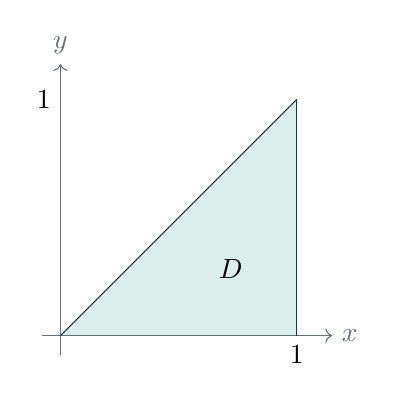
\begin{tikzpicture}[x=30mm,y=30mm]
    \fill[teal!15] (0,0)--(1,0)--(1,1)--cycle;
    \draw[->,muted] (-.08,0)--(1.15,0) node[right] {$x$};
    \draw[->,muted] (0,-.08)--(0,1.15) node[above] {$y$};
    \draw[navy] (0,0)--(1,1);
    \draw[navy] (1,0)--(1,1);
    \node at (.72,.28) {$D$};
    \node[below] at (1,0) {$1$};
    \node[left] at (0,1) {$1$};
  \end{tikzpicture}
  \end{center}

  \item 固定した \(t\in\R\) に対し、\((x,y)\mapsto e^{-ty}\) は
  有界閉領域 \(D\) 上の連続関数である。したがって
  \(\iint_D\abs{e^{-ty}}\,\dd x\dd y<\infty\) であり、
  Fubini の定理により積分順序を交換できる。
  また \(e^{-ty}\ge0\) なので、「非負なら積分値が有限かを先に確認しなくても
  順序交換できる」という Tonelli の定理からも交換できる。
  \[
  \begin{aligned}
  F(t)
  &=\int_0^1\int_0^x e^{-ty}\,\dd y\dd x\\
  &=\int_0^1\int_y^1 e^{-ty}\,\dd x\dd y
  =\boxed{\int_0^1(1-y)e^{-ty}\,\dd y}.
  \end{aligned}
  \]

  \item \(g(t,y)=(1-y)e^{-ty}\) とおく。
  \(g\) と
  \[
  g_t(t,y)=-y(1-y)e^{-ty}
  \]
  は任意の有界閉長方形
  \([t_0-1,t_0+1]\times[0,1]\) 上で連続である。
  よって積分記号の下で微分する定理を適用でき、
  \[
  \boxed{F'(t)=-\int_0^1y(1-y)e^{-ty}\,\dd y}.
  \]

  \item \(t=0\) を直接代入すると
  \[
  F(0)=\int_0^1(1-y)\,\dd y=\boxed{\frac12},
  \]
  \[
  F'(0)=-\int_0^1(y-y^2)\,\dd y
  =-\left(\frac12-\frac13\right)
  =\boxed{-\frac16}.
  \]
  \(t\ne0\) では部分積分により
  \[
  \int_0^1e^{-ty}\,\dd y=\frac{1-e^{-t}}t,
  \]
  \[
  \int_0^1ye^{-ty}\,\dd y
  =-\frac{e^{-t}}t+\frac{1-e^{-t}}{t^2}.
  \]
  差を取って
  \[
  \boxed{F(t)=\frac{t-1+e^{-t}}{t^2}}\qquad(t\ne0).
  \]
\end{enumerate}

\solutionhead{A2｜微分積分}{楕円上の変数変換}

\begin{enumerate}
  \item
  \[
  \frac{x^2}{a^2}+\frac{y^2}{b^2}
  =r^2(\cos^2\theta+\sin^2\theta)=r^2.
  \]
  従って楕円 \(D\) は
  \[
  0\le r\le1,\qquad 0\le\theta<2\pi
  \]
  に移る。Jacobian は
  \[
  \frac{\partial(x,y)}{\partial(r,\theta)}
  =\begin{vmatrix}
  a\cos\theta&-ar\sin\theta\\
  b\sin\theta&br\cos\theta
  \end{vmatrix}
  =ab r.
  \]
  \(a,b,r\ge0\) だから
  \[
  \boxed{\left|\frac{\partial(x,y)}{\partial(r,\theta)}\right|=ab r},
  \qquad
  \dd x\dd y=ab r\,\dd r\dd\theta.
  \]

  \item
  \[
  \iint_D1\,\dd x\dd y
  =ab\int_0^{2\pi}\int_0^1r\,\dd r\dd\theta
  =ab\cdot2\pi\cdot\frac12
  =\boxed{\pi ab}.
  \]

  \item \(x^2=a^2r^2\cos^2\theta\) なので
  \begin{align*}
  \iint_Dx^2\,\dd x\dd y
  &=a^3b
  \int_0^1r^3\,\dd r
  \int_0^{2\pi}\cos^2\theta\,\dd\theta\\
  &=a^3b\cdot\frac14\cdot\pi
  =\boxed{\frac{\pi a^3b}{4}}.
  \end{align*}

  \item \(x^2y^2=a^2b^2r^4\cos^2\theta\sin^2\theta\) なので
  \begin{align*}
  \iint_Dx^2y^2\,\dd x\dd y
  &=a^3b^3
  \int_0^1r^5\,\dd r
  \int_0^{2\pi}\cos^2\theta\sin^2\theta\,\dd\theta\\
  &=a^3b^3\cdot\frac16\cdot\frac\pi4
  =\boxed{\frac{\pi a^3b^3}{24}}.
  \end{align*}
\end{enumerate}

\begin{pointbox}[楕円の変数変換]
円の \(x=r\cos\theta,\ y=r\sin\theta\) を、\(x\) 方向に \(a\) 倍、
\(y\) 方向に \(b\) 倍したものが
\[
x=ar\cos\theta,\qquad y=br\sin\theta.
\]
面積要素にも同じ伸び \(ab\) が掛かるので、Jacobian は \(ab r\) になる。
\end{pointbox}

\solutionhead{T1｜集合と位相}{相対位相・コンパクト性・連結性}

\begin{enumerate}
  \item
  \[
  U=X\cap\bigl((0,\infty)\times\R\bigr).
  \]
  \((0,\infty)\times\R\) は \(\R^2\) の開集合なので、
  相対位相の定義から \(U\) は \(X\) の開集合である。

  一方、例えば \(p=(1/2,0)\in U\) とする。
  任意の \(r>0\) に対し
  \((1/2,r/2)\in B_{\R^2}(p;r)\) だが、この点は \(U\) に入らない。
  よって \(p\) を含み \(U\) に含まれる \(\R^2\) の開球はなく、
  \(U\) は \(\R^2\) では開でない。

  \item \([-1,1]\times\{0\}\) と \(\{0\}\times[-1,1]\) は
  \(\R^2\) の閉集合であり、その有限和集合 \(X\) も閉集合。
  また \(X\subset[-1,1]^2\) なので有界である。
  Heine--Borel の定理より
  \[
  \boxed{X\text{ はコンパクト}}.
  \]

  \item 任意の \(p,q\in X\) に対し
  \[
  \gamma(t)=
  \begin{cases}
  (1-2t)p,&0\le t\le1/2,\\
  (2t-1)q,&1/2\le t\le1
  \end{cases}
  \]
  とおく。各区間で連続で、\(t=1/2\) ではどちらも \((0,0)\) になるため
  \(\gamma:[0,1]\to X\) は連続。
  また \(\gamma(0)=p\)、\(\gamma(1)=q\) である。
  よって任意の二点を道で結べるので \(X\) は道連結、したがって連結。

  \item 次の四集合を考える。
  \[
  \begin{aligned}
  C_1&=(0,1]\times\{0\},&
  C_2&=[-1,0)\times\{0\},\\
  C_3&=\{0\}\times(0,1],&
  C_4&=\{0\}\times[-1,0).
  \end{aligned}
  \]
  各 \(C_j\) は区間と同相なので連結である。
  また \(Y=X\setminus\{(0,0)\}\) とおくと、
  例えば
  \[
  C_1=Y\cap\bigl((0,\infty)\times\R\bigr)
  \]
  であり \(Y\) の開集合である。補集合は残り三集合の和で同様に開だから、
  \(C_1\) は \(Y\) で閉でもある。他の \(C_j\) も同じ。
  従って異なる腕を含む連結集合は存在せず、
  \[
  \boxed{X\setminus\{(0,0)\}\text{ の連結成分は }C_1,C_2,C_3,C_4}.
  \]
\end{enumerate}

\begin{pointbox}[確認]
相対位相での開集合は必ず
\[
U=X\cap O\qquad(O\text{ は全体空間の開集合})
\]
と書いて示す。連結性は、具体的な道を一本書ければ最も速い。
\end{pointbox}

\solutionhead{T2｜集合と位相}{コンパクト空間から Hausdorff 空間への写像}

\begin{enumerate}
  \item \(Y\) を Hausdorff 空間、\(K\subset Y\) をコンパクト集合とする。
  \(p\in Y\setminus K\) を固定する。各 \(x\in K\) に対し、Hausdorff 性から
  \[
  x\in U_x,\qquad p\in V_x,\qquad U_x\cap V_x=\varnothing
  \]
  となる開集合 \(U_x,V_x\subset Y\) が取れる。

  \(\{U_x\}_{x\in K}\) は \(K\) の開被覆なので、コンパクト性から
  \(U_{x_1},\ldots,U_{x_m}\) で \(K\) を覆える。そこで
  \[
  U=\bigcup_{j=1}^mU_{x_j},
  \qquad
  V=\bigcap_{j=1}^mV_{x_j}
  \]
  とおく。\(U,V\) は開、\(K\subset U\)、\(p\in V\)、かつ
  \(U\cap V=\varnothing\)。
  従って \(V\subset Y\setminus K\)。任意の \(p\in Y\setminus K\) が
  \(Y\setminus K\) に含まれる開近傍を持つので、\(Y\setminus K\) は開である。
  よって
  \[
  \boxed{K\text{ は }Y\text{ の閉集合}}.
  \]

  \item \(F\subset X\) を任意の閉集合とする。
  \(X\) はコンパクトだから \(F\) もコンパクトであり、連続性から
  \(f(F)\) は \(Y\) のコンパクト集合である。(1) より \(f(F)\) は \(Y\) で閉じている。

  \(f\) は全単射なので逆写像が存在し、
  \[
  (f^{-1})^{-1}(F)=f(F).
  \]
  任意の閉集合 \(F\subset X\) の逆像が \(Y\) で閉じているから
  \[
  \boxed{f^{-1}:Y\to X\text{ は連続}}.
  \]

  \item まず \(0\sim1\) であり
  \[
  (\cos0,\sin0)=(\cos2\pi,\sin2\pi)
  \]
  なので \(h([t])\) は代表元の取り方によらず、正しく定義される。
  また円周上の各点には角度 \(2\pi t\ (0\le t<1)\) が一意に対応するため、
  \(h\) は全単射である。

  写像
  \[
  h\circ q:[0,1]\to S^1,
  \qquad
  t\longmapsto(\cos2\pi t,\sin2\pi t)
  \]
  は連続である。\(Z\) には \(q\) による商位相が入っているので、
  \(h\circ q\) の連続性から \(h\) は連続である。

  \([0,1]\) はコンパクトで、\(q\) は連続な全射だから
  \(Z=q([0,1])\) はコンパクトである。一方、\(S^1\subset\R^2\) は
  Hausdorff 空間である。従って (2) を \(h:Z\to S^1\) に適用でき、
  \(h^{-1}\) も連続である。ゆえに
  \[
  \boxed{Z\text{ と }S^1\text{ は同相}}.
  \]
\end{enumerate}

\begin{pointbox}[証明のつながり]
\[
\begin{array}{c}
X\text{ がコンパクト}\\[-1mm]
F\subset X\text{ が閉}
\end{array}
\Longrightarrow
F\text{ がコンパクト}
\Longrightarrow
f(F)\text{ がコンパクト}
\overset{Y\text{ Hausdorff}}{\Longrightarrow}
f(F)\text{ が閉}.
\]
従って \(f\) は閉写像となり、全単射なら逆写像が連続になる。
\end{pointbox}

\clearpage
\thispagestyle{empty}
\vspace*{20mm}
{\color{navy}\bfseries\Large 最後に確認する式}\par
\vspace{2mm}{\color{navy}\rule{\linewidth}{.7pt}}\vspace{4mm}

\[
\dim V=\dim\Ker T+\dim\Img T,
\qquad
A\text{ が対角化可能}
\iff\sum_\lambda\dim\Ker(A-\lambda I)=n.
\]

\[
x=r\cos\theta,\quad y=r\sin\theta,\quad
\dd x\dd y=r\,\dd r\dd\theta.
\]

\[
\frac{\dd}{\dd x}\int_{\phi(x)}^{\psi(x)}f(x,y)\,\dd y
=f(x,\psi(x))\psi'(x)-f(x,\phi(x))\phi'(x)
+\int_{\phi(x)}^{\psi(x)}f_x(x,y)\,\dd y.
\]

\[
d(x,A)=\inf_{a\in A}d(x,a),
\qquad
\abs{d(x,A)-d(y,A)}\le d(x,y).
\]

\[
W\le V
\iff
W\ne\varnothing,\quad
au+bv\in W
\quad(u,v\in W,\ a,b\in\F).
\]

\vfill
\begin{center}
\color{muted}
定義を書く。使う定理の仮定を書く。最後に問われた結論を一文で書く。
\end{center}


\end{document}
